\documentclass[11pt,oneside,openany]{article}

\usepackage{graphicx}
\usepackage{color}    % to define macros for colors
\usepackage{listings} % package to include source code

\author{Matteo Franchin}

%TYPESETTING:----------------------------------------------------------

% Reset page margins properly for doublesided pages

% No headings
\pagestyle{plain}

% 1.5 interline spacing --> corresponds to linespread 1.3
% 2.0 interline spacing --> corresponds to linespread 1.6
\linespread{1.3}

\setlength{\marginparwidth}{0mm}
\setlength{\marginparsep}{0mm}
\setlength{\oddsidemargin}{0.7in} % corresponds to 1 + 0.7 = 1.7 inches
\setlength{\evensidemargin}{0.7in} % corresponds to 1.7 inches
\setlength{\textwidth}{145mm}
\setlength{\textheight}{220mm}
\setlength{\voffset}{-20mm}
\raggedbottom

%----------------------------------------------------------------------
% Extra colors

\definecolor{lightgrey}{cmyk}{0.05,0.05,0.05,0}
\definecolor{gray}{rgb}{0.5,0.5,0.5}

%----------------------------------------------------------------------
% Style for code listings

\lstdefinestyle{defaultstyle}{}
\lstset{language=Python}
\lstset{basicstyle=\ttfamily\scriptsize}
\lstset{showstringspaces=false}
\lstset{keywordstyle=\color{blue}}
\lstset{stringstyle=\color{red}}
\lstset{commentstyle=\color{gray}\emph}
\lstset{numbers=left,frame=single}
\lstset{backgroundcolor=\color{lightgrey}}

\newcommand{\vect}[1]{\mathbf{#1}}
\newcommand{\vecs}[2]{\mathbf{#1_{\mathrm{#2}}}}
\newcommand{\vm}{\vect{m}}
\newcommand{\vM}{\vect{M}}

\begin{document}

\titlepage

\section{The Slonczewski Spin Transfer Torque in Nmag5}
In this document we explain how to use Nmag5 to run simulations which
include the spin transfer torque (Slonczewski model). This is particular
useful to simulate spin valves. We notice that Nmag5 implements the same
term which is implemented in OOMMF 1.2a4 (extension \verb|Oxs_SpinXferEvolve|
in \verb|oommf/app/oxs/local/spinxferevolve.cc| where \verb|oommf| is the
directory produced untarring the tarball). Notice that OOMMF comes with some
\verb|mif| example files where the extension is used.

It may be useful to know that the term we implement \emph{is not} the one
described in the original paper that Slonczewski wrote/submitted in 1996
(J. C. Slonczewski, J. Magn. Magn. Mater. 159, L1 (1996)).
The term we implement was theoretically described in 2004
in [J. Xiao, \emph{et. al.}, Phys. Rev. B, 70, 172405 (2004)].
This paper generalised what was derived by Slonczewski in 2002
[J. C. Slonczewski, J. Magn. Magn. Mater. 247, 324 (2002)].
A clearer formulation of the equations can be found in OOMMF user guide
(\verb|oommf/doc/userguide/userguide.pdf|).

Below we provide the Landau-Lifshitz-Gilbert with the additional STT term
included (as given in the OOMMF user guide):
\begin{equation}
  \frac{d\vm}{dt} = -|\gamma|\,\vm\times\vecs{H}{eff}
   + \alpha
     \left(\vm\times\frac{d\vm}{dt}\right)
   + |\gamma|\beta\epsilon
     \left(\vm\times\vm_p\times\vm\right)
   - |\gamma|\beta\epsilon^\prime\,\vm\times\vm_p,
\label{eq:oxsllgspinxfer}
\end{equation}
where
\begin{eqnarray*}
\vm & = & \mbox{reduced magnetization, $\vM/M_s$} \\
\gamma & = & \mbox{Gilbert gyromagnetic ratio} \\
\beta & = & \left|\frac{\hbar}{\mu_0 e}\right|\frac{J}{t M_s} \\
\vm_p & = & \mbox{(unit) electron polarization direction} \\
\epsilon & = &
\frac{P\Lambda^2}{(\Lambda^2+1)+(\Lambda^2-1)(\vm\cdot\vm_p)} \\
\epsilon^\prime & = & \mbox{secondary spin tranfer term}.
\end{eqnarray*}
In the definition of $\beta$, $e$ is the electron charge in C, $J$ is
current density in A/m${}^2$, $t$ is the free layer thickness in meters,
and $M_s$ is the saturation magnetization in A/m.

Note that, in the Nmag implementation we take $\epsilon^\prime = 0$.
We also have the following correspondences:

\begin{tabular}{ll}
$P$ & \verb|MagMaterial.sl_P| \\
$\lambda$ & \verb|MagMaterial.sl_lambda| \\
$t$ & \verb|MagMaterial.sl_d| \\
$\vecs{m}{P}$ & \verb|Simulation.model.quantities["sl_fix"]| \\
$J$ & \verb|Simulation.model.quantities["sl_current_density"]| \\
\end{tabular}

\subsection{Example: dynamics of a disk excited by a sinc pulse}
We now show an example where we use the extension to model the dynamics
in a spin valve.
The system geometry is shown in Fig. \ref{fig:sketch}.
%
\begin{figure}[h]
\begin{center}
%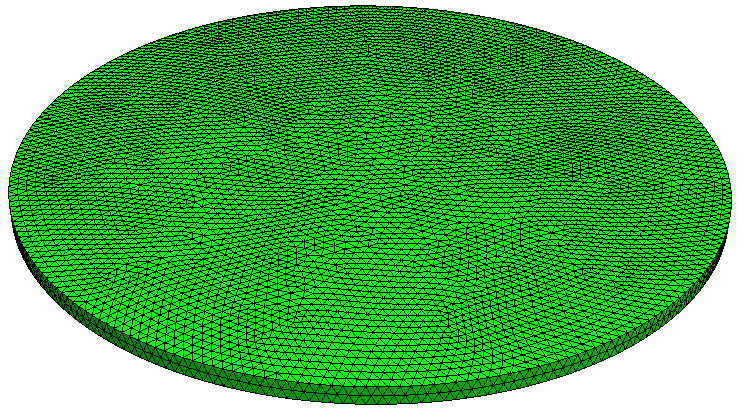
\includegraphics[width=10.0cm]{disk}
\caption[Sketch]{A sketch of the system modeled in the simulation.}
\label{fig:mesh}
\end{center}
\end{figure}
%
The simulation script is split in the two figures Fig. \ref{fig:script1of2} and
\ref{fig:script2of2}. 

\begin{figure}[!p]
\lstinputlisting[linerange=1-39]{../../slonczewski/validation/nmag/run.py}
\caption{Part 1.}
\label{fig:script1of2}
\end{figure}

\begin{figure}[!h]
\lstinputlisting[linerange=40-60,firstnumber=40]{../../slonczewski/validation/nmag/run.py}
\caption{Part 2.}
\label{fig:script2of2}
\end{figure}

We will now describe the script line-by-line:

\textbf{Lines 1-6:} these are the usual import statements, which often occur
in Nmag scripts. Notice the nmag5 specific imports (\verb|from nmag.nmag5|
\verb|import| $\ldots$ and \verb|from| \verb|nsim.model import| $\ldots$).

\textbf{Lines 7-12:} these lines define some useful variables such as
\verb|ps| for picosecond, \verb|nm| for nanometre.  The also define the
spherical angles for the polarisation direction \verb|theta| and \verb|phi|,
the size of the mesh, the applied current density and the applied field
(in milli-Tesla).

\textbf{Lines 13-21:} if the mesh \verb|film.nmesh.h5| does not exist, then
we create it, by using the \verb|netgen_mesh_from_string| function from the
\verb|nsim.netgen| module. Note that we provide the geo file as a Python
string. The function does automatically invoke Netgen (which must be installed
on the system) and does convert automatically the Neutral output to the
Nsim \verb|nmesh.h5| file format.

\textbf{Lines 22-30:} the material is defined, together with its anisotropy
parameters.

\textbf{Lines 31-34:} Other three STT-related parameters are defined for the
material. Notice that here the interface is not polished and the material
parameters are added just as attributes of the material \verb|mat|. (we should
repair this, either by adding these extra parameters to the \verb|MagMaterial|
class or by accepting a \verb|**kwargs| in \verb|MagMaterial|.

\textbf{Lines 35-38:} the function \verb|setup_simulation| is used to create
the materials, create the simulation object and load the mesh. These operations
are collected together in this function, as they are needed twice: once for the
relaxation simulation and a second time for the dynamics simulation.  Notice,
how the tolerances are set. Controlling all the tolerances is very important in
this kind of simulations, where accuracy can substantially improve the
results. The function \verb|setup_simulation| returns the simulation object, so
it can be further manipulated after the function has been called.

\textbf{Lines 39-50:} Other STT-related quantities are set. In particular,
the direction of the polarisation \verb|P_direction| is computed from the
polar angles and it is used to set the vector \verb|sl_fix|.
The value of the current density is also set. 

\textbf{Lines 51-57:} The tolerances for the simulation are set
and the relaxation is launched, saving the averages every 5 picoseconds.
Notice that the stopping criterion is disabled (\verb|stopping_dm_dt| is set
to zero) and the simulation is forced to quit after 10 nanoseconds
(\verb|do=[("exit", at("time", 10000*ps))])|).
Notice also that the method \verb|Simulation.set_params| is capable
of setting the demag tolerances \verb|demag_..._tol| and the preconditioner
tolerances \verb|ts_pc_..._tol|. This is a new feature of Nmag5 (and is
not yet available in Nmag4, where one needs to provide these tolerances
in a dictionary passed to the \verb|Simulation| object during creation,
which also means that one cannot change them later on in the simulation).


%
%\lstinputlisting[linerange=87-87,firstnumber=87]{script.py}
%

\subsection{Results}
In Fig. \ref{fig:mif1of2} and \ref{fig:mif2of2} we provide the OOMMF script
which implements the same simulation we described for Nmag.

\begin{figure}[!p]
  \lstinputlisting[language=tcl,linerange=1-47]%
  {../../slonczewski/validation/oommf/run.mif}
\caption{Part 1.}
\label{fig:mif1of2}
\end{figure}

\begin{figure}[!h]
  \lstinputlisting[language=tcl,linerange=48-89,firstnumber=48]%
  {../../slonczewski/validation/oommf/run.mif}
\caption{Part 2.}
\label{fig:mif2of2}
\end{figure}

The comparison of the results is shown in Fig. \ref{fig:results}.

\begin{figure}[!h]
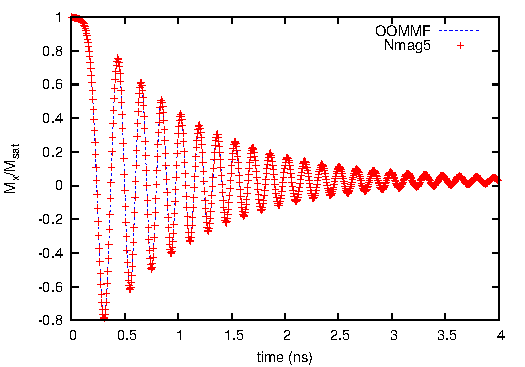
\includegraphics[width=10.0cm]{plot}
\caption{Comparison between the OOMMF and the Nmag implementation of the STT.
  The plot shows the time dependency of the $x$ component of the normalised
  magnetisation. Note that in the simulation the demag is disabled (the
  agreement is then expected to be very good, as it does not depend
  on the spatial discretisation).}
\label{fig:results}
\end{figure}

\subsection{Final remarks}
As stated before, the term implemented in OOMMF and Nmag is not the one
given in the paper published in the 1996 [JMMM 159 (1996)]. It is a more
recent model, result of the work of Slonczewski [JMMM 247 (2002)] with the
extensions from Xiao [PRB 70, 172405 (2004)]. This model requires the user
to give, beside the polarization $P$, also another quantity $\lambda^2$.
It can be seen from the mathematics, that taking:
$$
P = a/(2 - 2a) \mathrm{ and } \lambda^2 = (2 - 2a)/(1 - 2a),
$$
where $a = 4 (sqrt(P_0)/(1 + P_0))^3$ and P0 is the polarisation in the
Slonczewski model, the Xiao model reduces to the Slonczewski model.
\end{document}
